% Written by paper/figures/src/v6_gallery.py; edit the script, not this file.
\begin{figure}[p]
  \centering
  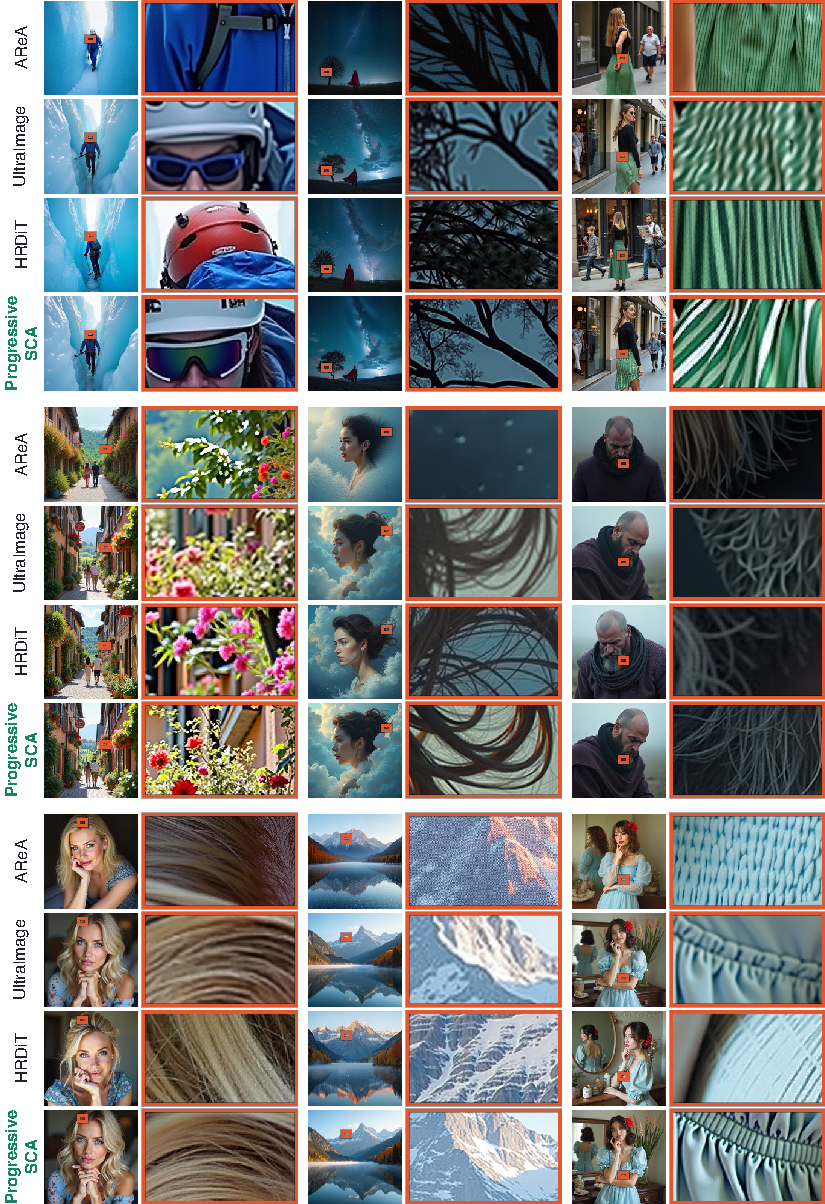
\includegraphics{figures/v6/gallery_prog16.pdf}
  \caption{\textbf{Progressive \sca{} keeps the native detail that AReA and UltraImage blur (prompts 1 to 9 of 18).} Evaluation prompts outside Figures~\ref{fig:qual_prog} and~\ref{fig:gallery_prog}, chosen by a fixed seed (seed 16); seed 0 for every image. Each crop shows native pixels of the window that maximises the smallest edge energy among the four methods. Figure~\ref{fig:gallery_prog16b} continues.}
  \label{fig:gallery_prog16}
\end{figure}
\begin{figure}[p]
  \centering
  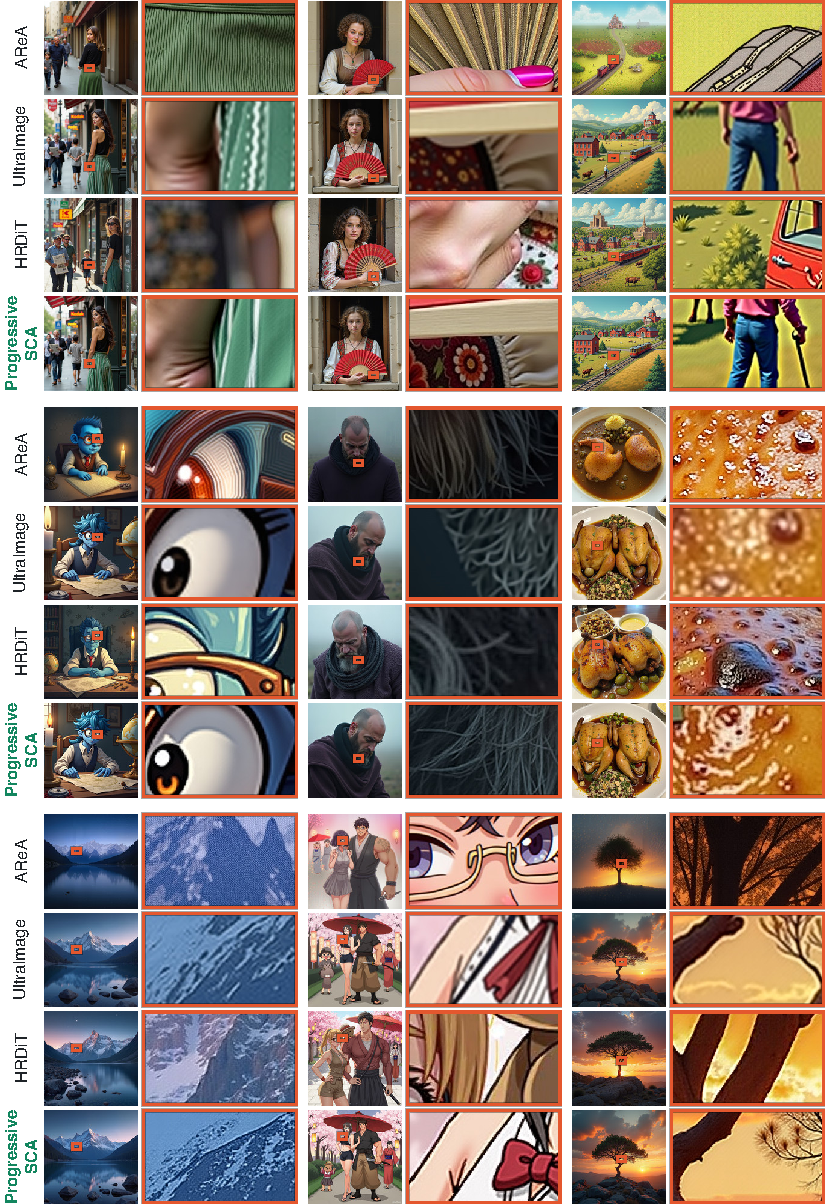
\includegraphics{figures/v6/gallery_prog16b.pdf}
  \caption{\textbf{Progressive \sca{} keeps the native detail that AReA and UltraImage blur (prompts 10 to 18 of 18).} Evaluation prompts outside Figures~\ref{fig:qual_prog} and~\ref{fig:gallery_prog}, chosen by a fixed seed (seed 16); seed 0 for every image. Each crop shows native pixels of the window that maximises the smallest edge energy among the four methods.}
  \label{fig:gallery_prog16b}
\end{figure}
